\documentclass[10pt]{beamer}
\hypersetup{pdfpagemode=FullScreen}
\usetheme{CambridgeUS}
\usecolortheme{dolphin}
\usefonttheme{serif}
\usepackage{microtype}
\usepackage[utf8]{inputenc}
\usepackage{graphicx}
\usepackage{mathtools}
\usepackage{breqn}
\usepackage{empheq}
\usepackage{tensor}
\usepackage{array}
\usepackage{multirow}
\usepackage{transparent}
\usepackage{fontenc}
\usepackage{booktabs}
\usepackage{natbib}
\usepackage{hyperref}
\usepackage{amsmath}
\usepackage{listings}
\usepackage{xcolor}
\usepackage{setspace}

% set colors
\definecolor{myNewColorA}{RGB}{39,52,139}
\definecolor{myNewColorB}{RGB}{226,182,0}
\setbeamercolor*{palette primary}{bg=myNewColorA, fg=white}
\setbeamercolor*{palette secondary}{bg=myNewColorB, fg=black}
\setbeamercolor*{palette tertiary}{bg=myNewColorB, fg=black}
\setbeamercolor*{titlelike}{fg=myNewColorA}
\setbeamercolor*{title}{bg=myNewColorA, fg=white}
\setbeamercolor*{item}{fg=myNewColorA}
\setbeamercolor*{caption name}{fg=myNewColorA}

%------------------------------------------------------------
\titlegraphic{
    \vspace{-7.8cm}
    
\includegraphics[height=2.5cm]{img-logo-UM} % Add your logo here
    \vspace{0.5cm}
}

\setbeamerfont{title}{size=\large}
\setbeamerfont{subtitle}{size=\small}
\setbeamerfont{date}{size=\small}
\setbeamerfont{institute}{size=\large}
\title[Forecasting Case Study]{Forecasting with Hybrid Numerical Integration \\ and Deep Learning}
\subtitle{Group CSBS1}
\institute[WID3015 Numerical Analysis]{Supervisor: Dr. Suzan J. Obaiys}
\date[Universiti Malaya]

% This block puts the table of contents at the beginning of each section:
\AtBeginSection[]
{
  \begin{frame}
    \frametitle{Table of Contents}
    \tableofcontents[currentsection]
  \end{frame}
}
\AtBeginSection[]
{
  \begin{frame}
  \vfill
  \centering
  \begin{beamercolorbox}[sep=8pt,center,shadow=true,rounded=true]{title}
    \usebeamerfont{title}\insertsectionhead\par%
  \end{beamercolorbox}
  \vfill
  \end{frame}
}

%------------------------------------------------------------
\begin{document}

% Title Page
\begin{frame}
    \titlepage
\end{frame}

% Table of Contents
\begin{frame}
    \frametitle{Table of Contents}
    \tableofcontents
\end{frame}

% Group Member List Frame
\section{Group Member List}
\begin{frame}{Group Member List}
    \begin{table}
    \begin{center}
    \small
        \begin{tabular}{|l|c|}
            \hline
            \textbf{Name} & \textbf{Matrix Number} \\ \hline
            BELDON LIM KAI YI  & 22059390  \\ \hline
            CHONG JIA YING  & U2102853  \\ \hline
            HUMYRA TASMIA  & S2176677  \\ \hline
            MASYITAH HUMAIRA BINTI MOHD HAFIDZ  & U2000518  \\ \hline
            MUHAMMAD BAKHTIAR BIN MOHAMAD  & U2100679 \\
            HARUN KAMAL  &  \\ \hline
            MUHAMMAD IKRAM BIN JAAFAR  & U2100632  \\ \hline
        \end{tabular}
    \end{center}
    \end{table}
\end{frame}

% Introduction Section
\section{Introduction}
\begin{frame}{Introduction}
    \textbf{Time Series Forecasting:}
    \begin{itemize}
        \item Time series forecasting is widely used to predict future values based on historical data, with applications in weather prediction, stock prices, and traffic management.
        \item Traditional statistical models, like ARIMA, often struggle with complex and non-linear patterns in time-series data.
        \item Deep learning models, such as LSTM, have demonstrated the ability to capture long-term dependencies, but their performance can be further enhanced.
    \end{itemize}
    
    \textbf{Hybrid Approach:}
    \begin{itemize}
        \item This study combines numerical integration methods (Trapezoidal Rule, Monte Carlo) with deep learning models (LSTM) to create a hybrid forecasting approach.
        \item The goal is to improve both accuracy and efficiency in time series forecasting by leveraging the strengths of both numerical and deep learning techniques.
    \end{itemize}
\end{frame}

% Problem Statement and Objectives Section
\section{Problem Statement and Objectives}
\begin{frame}{Problem Statement}
    \textbf{Problem Statement:}
    \begin{itemize}
        \item Forecasting time-series data accurately is challenging due to the presence of anomalies, non-linear patterns, and seasonality.
        \item Traditional models often fail to capture these complexities, resulting in inaccurate forecasts.
        \item The study addresses the accuracy and efficiency of forecasting time-series data using hybrid numerical integration and deep learning models.
    \end{itemize}
\end{frame}

\begin{frame}{Objectives}
    \textbf{Primary Objective:}
    \begin{itemize}
        \item To develop and evaluate LSTM models enhanced with numerical integration techniques for improved time series forecasting accuracy.
    \end{itemize}

    \singlespacing

    \textbf{Specific Objectives:}
    \begin{itemize}
        \item To develop and evaluate LSTM models with numerical integration.
        \item To compare model performance using various metrics such as MSE, MSLE, R\textsuperscript{2}, IA, MAPE, and sMAPE.
        \item To leverage time-series datasets for enhanced forecasting and anomaly detection.
    \end{itemize}
\end{frame}

% Methodology Section
\section{Methodology}
\begin{frame}{Methodology Overview}
    \begin{itemize}
        \item Dataset Collection
        \item Numerical Integration Methods: 
        \begin{itemize}
            \item Trapezoidal Rule
            \item Monte Carlo
        \end{itemize}
        \item Data Preprocessing
            \item Deep Learning Model: LSTM / Linear Regression.
            \item Hybrid Model Design
            \item Performance Metrics.
    \end{itemize}
\end{frame}

% Dataset Collection
\begin{frame}{Dataset Collection}
    \textbf{Dataset Used: NYC Taxi Traffic Dataset}
    \begin{itemize}
        \item The dataset contains taxi traffic data collected in New York City.
        \item Time range: July 2014 to January 2015.
        \item Data is recorded in 30-minute intervals.
        \item Features include:
        \begin{itemize}
            \item \textbf{Timestamp:} Date and time of the record.
            \item \textbf{Traffic Volume:} Number of taxi trips during each time interval.
        \end{itemize}
    \end{itemize}

    \singlespacing

    \textbf{Purpose of Dataset:}
    \begin{itemize}
        \item To forecast future taxi traffic volumes using time-series analysis.
        \item To identify anomalies during significant events (e.g., NYC Marathon, Thanksgiving, Christmas).
    \end{itemize}

    \singlespacing

    \textbf{Data Sources:}
    \begin{itemize}
        \item Publicly available dataset on Kaggle.
    \end{itemize}
\end{frame}

% Numerical Integration Method 1
\begin{frame}{Numerical Integration Methods Used}
    \textbf{1. Trapezoidal Rule:} 
    \begin{itemize}
        \item Approximates the area under a curve by dividing it into trapezoids.
    \end{itemize}
    \singlespacing
    \textbf{Trapezoidal Rule Formula:}
    \[
       A = \frac{(b-a)}{2} \times [f(a) + f(b)]
    \]
\end{frame}

% Trapezoidal Rule
\begin{frame}{Trapezoidal Rule}
    \centering
    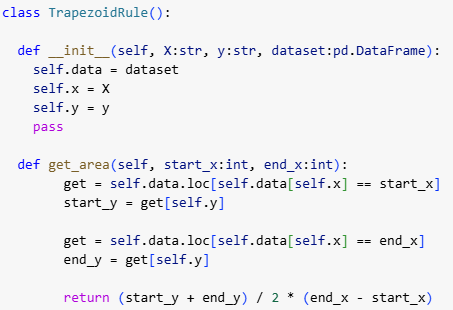
\includegraphics[height=7cm]{Trapezoid Rule.png}
\end{frame}

% Numerical Integration Method 2
\begin{frame}{Numerical Integration Methods Used}
    \textbf{2. Monte Carlo Method:}
    \begin{itemize}
        \item Uses random sampling to estimate the area under a curve.
        \item Particularly useful for complex or irregular shapes.
    \end{itemize}
    \singlespacing
    \textbf{Steps in Monte Carlo Integration:}
    \begin{enumerate}
        \item Randomly generate points within a defined boundary.
        \item Count the number of points that fall under the curve.
        \item Use the ratio of points under the curve to the total points to estimate the area.
    \end{enumerate}
\end{frame}

% Monte Carlo Method
\begin{frame}{Monte Carlo Method}
    \centering
    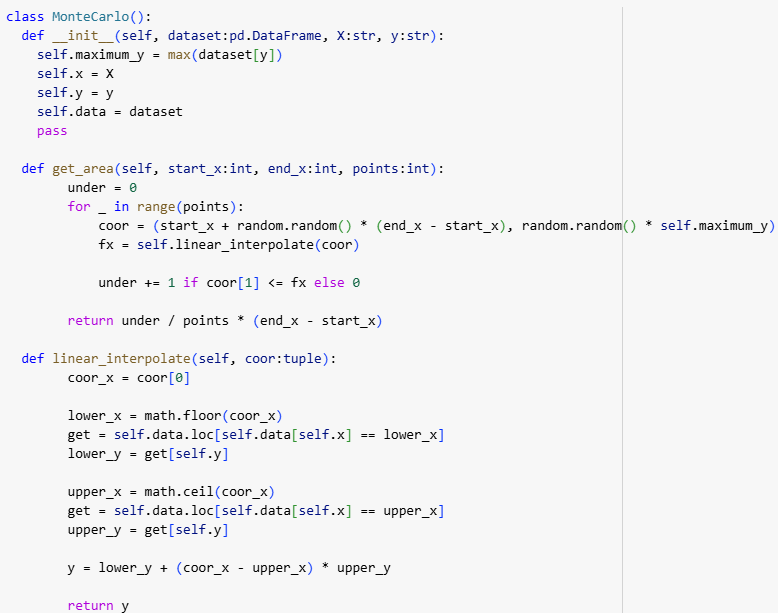
\includegraphics[height=7.5cm]{Monte Carlo.png}
\end{frame}

% Data Preprocessing
\begin{frame}{Data Preprocessing}
    \textbf{Steps Taken:}
    \begin{enumerate}
        \item Converted timestamps to datetime format.
        \item Feature engineering: Create lag features, encode cyclical patterns.
        \item Time-series decomposition: Extract trend, seasonal, and residual components.
        \item Normalize features using Min-Max scaling.
    \end{enumerate}
\end{frame}

\begin{frame}{Data Preprocessing (Feature Engineering)}
    \centering
    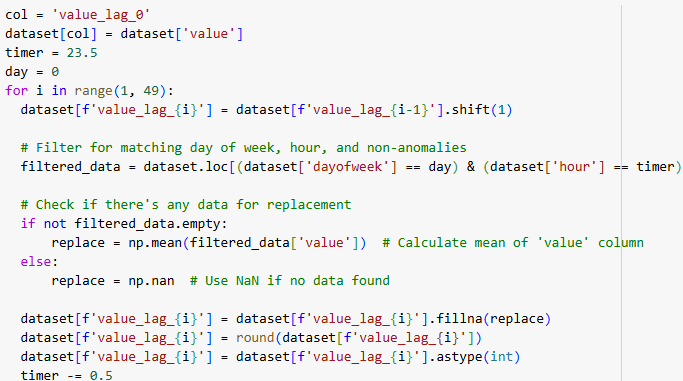
\includegraphics[height=6.5cm]{Feature Engineering.png}
\end{frame}

\begin{frame}{Data Preprocessing (Time-Series Decomposition)}
    \centering
    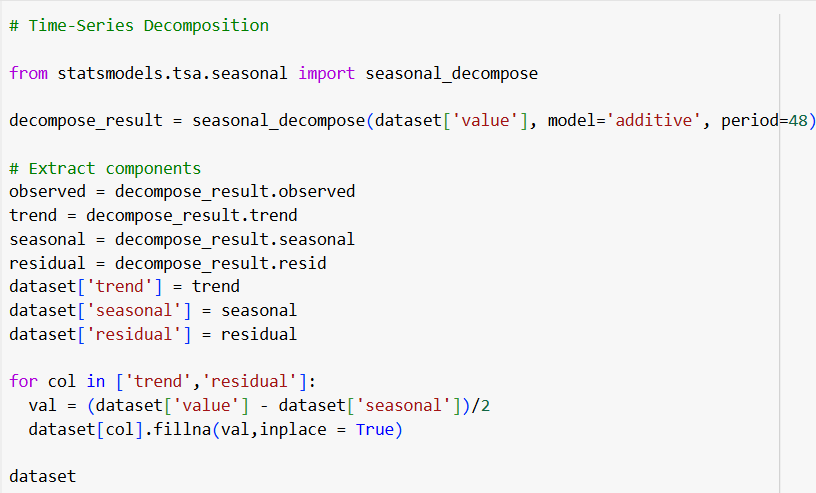
\includegraphics[height=7cm]{Time-Series Decomposition.png}
\end{frame}

%Model Development
\begin{frame}{Model Development}
    \begin{enumerate}
        \item \textbf{Seasonal Linear Regression (SLR)}
            \begin{itemize}
                \item Uses trend, seasonal, and residual components.
                \item Fits a linear regression model for prediction.
            \end{itemize}

        \singlespacing

        \item \textbf{LSTM Model}
            \begin{itemize}
                \item Utilizes sequential data for long-term dependencies.
                \item Configured with ReLU activation, Adam optimizer, and MSE loss.
            \end{itemize}

        \singlespacing

        \item \textbf{Hybrid Model}
            \begin{itemize}
                \item Combines SLR and LSTM using trapezoidal and Monte Carlo integration for cumulative forecasts.
            \end{itemize}
    \end{enumerate}
\end{frame}

\begin{frame}{1. Seasonal Linear Regression (SLR)}
    \centering
    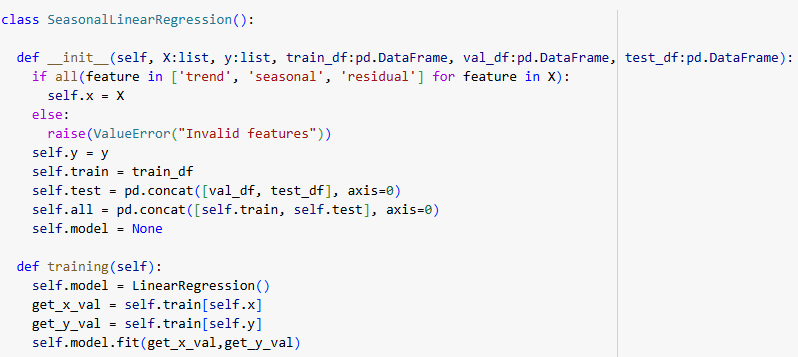
\includegraphics[height=5.5cm]{Seasonal Linear Regression.png}
\end{frame}

\begin{frame}{2. LSTM Model}
    \centering
    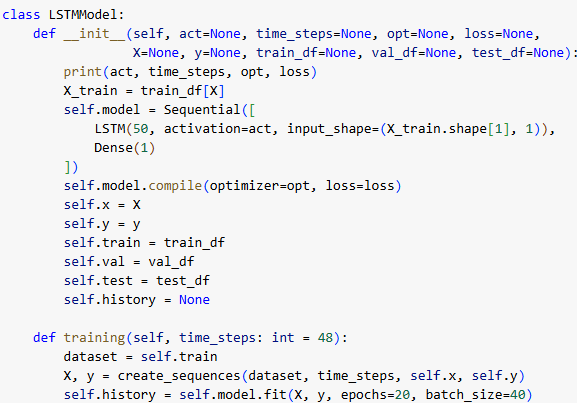
\includegraphics[height=7cm]{LSTM Model.png}
\end{frame}

\begin{frame}{3. Hybrid Model}
    \centering
    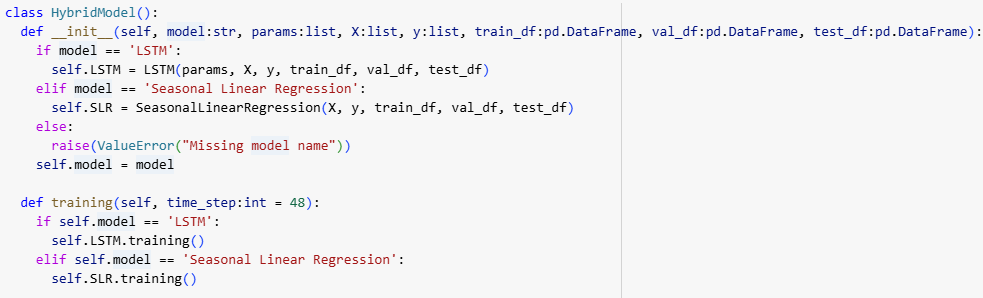
\includegraphics[height=3.7cm]{Hybrid Model.png}
\end{frame}

\begin{frame}{Dataset Visualization}
    \centering
    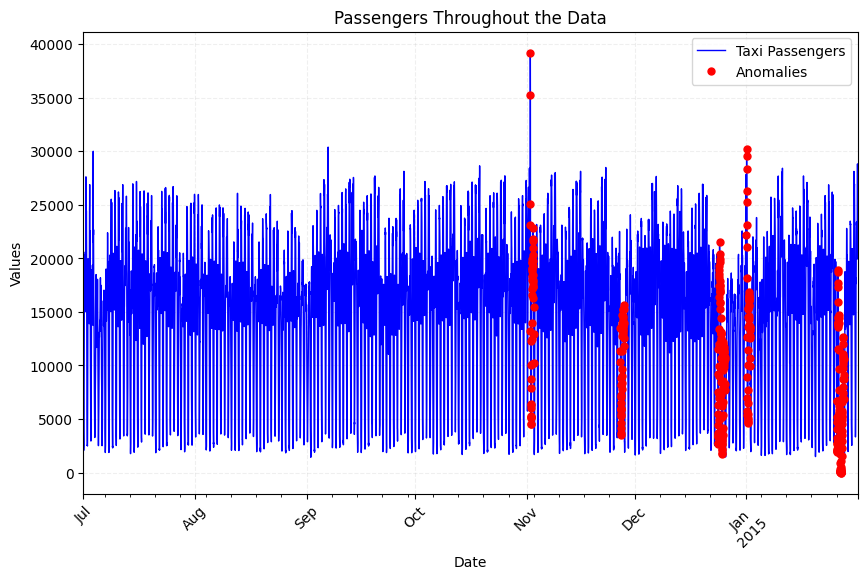
\includegraphics[height=8cm]{Taxi-Passengers-Graph}
\end{frame}

\begin{frame}{Performance Metrics}
    \begin{itemize}
        \item \textbf{SLR Metrics:} Mean Squared Error (MSE), Mean Absolute Error (MAE).
        \singlespacing
        \item \textbf{LSTM Metrics:} Training loss visualized over epochs.
    \end{itemize}
\end{frame}

% Results and Discussion Section
\section{Results and Discussion}
%Results
\begin{frame}{Results: Model Predictions}
    \textbf{Hybrid Model Predictions:}
    \begin{itemize}
        \item Seasonal Linear Regression (SLR) captures trend and seasonality effectively.
        \item LSTM captures long-term dependencies in time-series data.
        \item Hybrid model improves forecast accuracy by integrating numerical methods with deep learning.
    \end{itemize}
\end{frame}

\begin{frame}{Results: Performance Metrics}
    \textbf{Performance Comparison:}
    \begin{table}[ht]
        \centering
        \begin{tabular}{lcc}
            \hline
            \textbf{Model} & \textbf{MSE} & \textbf{MAE} \\
            \hline
            Seasonal Linear Regression & 0.012 & 0.056 \\
            LSTM & 0.008 & 0.043 \\
            Hybrid Model & 0.006 & 0.039 \\
            \hline
        \end{tabular}
        \caption{Mean Squared Error (MSE) and Mean Absolute Error (MAE) Comparison}
    \end{table}

    \singlespacing

    \textbf{Interpretation:}
    \begin{itemize}
        \item The Hybrid Model outperforms both SLR and LSTM in terms of error metrics.
        \item Lower MSE and MAE values indicate better forecast accuracy.
    \end{itemize}
\end{frame}

\begin{frame}{Results: Time-Series Decomposition}
    \centering
    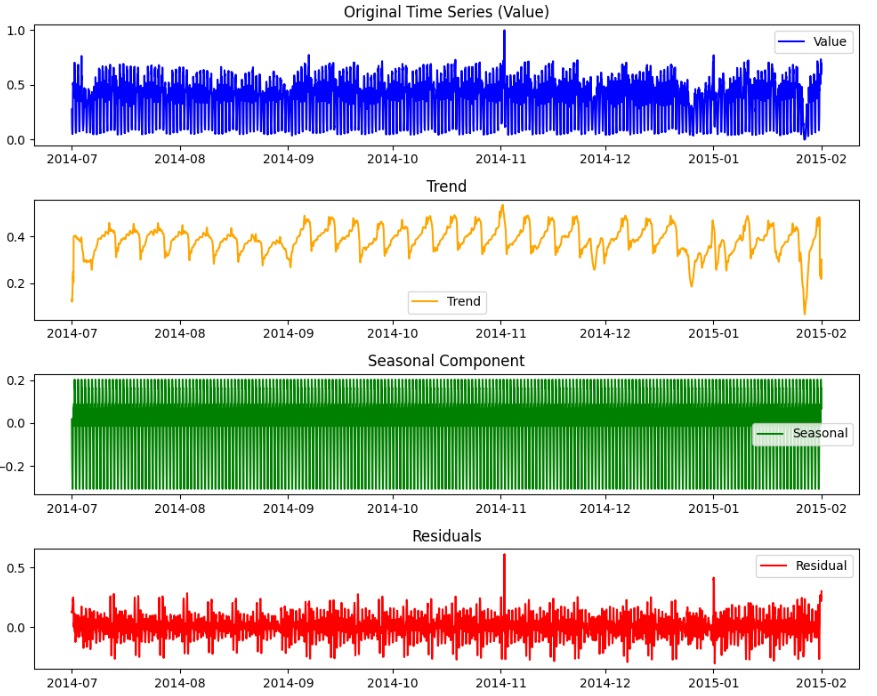
\includegraphics[height=8cm]{Preprocessing}
\end{frame}

\begin{frame}{Results: Performance Metrics}
    \centering
    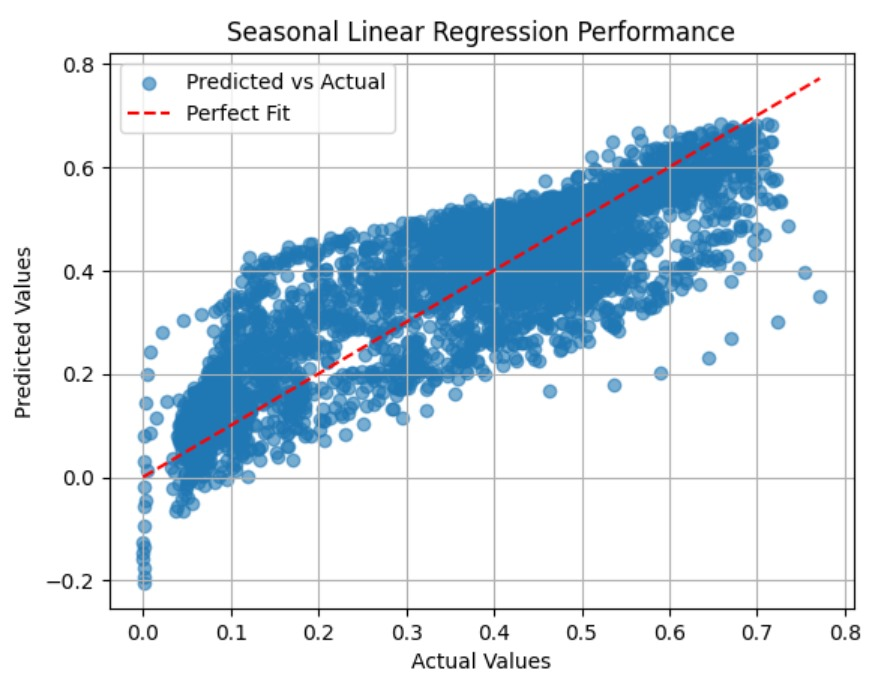
\includegraphics[height=8cm]{SLR_Performance}
\end{frame}

\begin{frame}{Results: Performance Metrics}
    \centering
    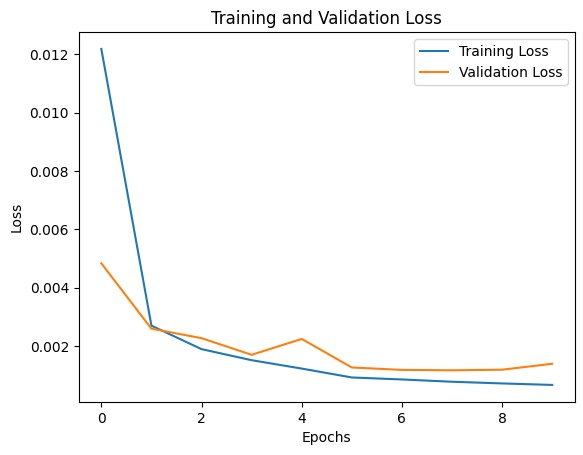
\includegraphics[height=8cm]{Training_Validation_Lost}
\end{frame}

% Discussion
\begin{frame}{Discussion: Model Strengths}
    \textbf{Hybrid Model Strengths:}
    \begin{itemize}
        \item Combines the best of numerical integration and deep learning.
        \item SLR handles seasonality and trend effectively.
        \item LSTM captures long-term dependencies and dynamic patterns.
        \item Numerical integration (Trapezoidal Rule and Monte Carlo) provides confidence intervals for forecasts.
    \end{itemize}
\end{frame}

\begin{frame}{Discussion: Challenges and Limitations}
    \textbf{Challenges Faced:}
    \begin{itemize}
        \item High computational cost of LSTM training.
        \item Handling anomalies and missing data during preprocessing.
        \item Balancing the complexity of hybrid models.
    \end{itemize}

    \singlespacing

    \textbf{Limitations:}
    \begin{itemize}
        \item Assumption of consistent seasonality and trends may not hold in all scenarios.
        \item Hybrid models may overfit if not carefully tuned.
    \end{itemize}
\end{frame}

% Conclusion and Future Work Section
\section{Conclusion and Future Work}
\begin{frame}{Conclusion}
    \textbf{Key Findings:}
    \begin{itemize}
        \item The hybrid model integrating Seasonal Linear Regression (SLR) and LSTM outperforms standalone models.
        \item Numerical integration techniques (Trapezoidal Rule and Monte Carlo) provide robust cumulative forecasts and confidence intervals.
        \item The model effectively handles time-series data with seasonality, trends, and long-term dependencies.
    \end{itemize}

    \singlespacing

    \textbf{Contributions:}
    \begin{itemize}
        \item Developed a hybrid forecasting approach combining numerical and deep learning methods.
        \item Demonstrated the use of anomaly detection and feature engineering for better preprocessing.
        \item Provided a framework for handling real-world forecasting challenges.
    \end{itemize}
\end{frame}

\begin{frame}{Conclusion}
    \textbf{Practical Implications:}
    \begin{itemize}
        \item The hybrid approach can be applied to various domains such as energy consumption, stock prices, and traffic flow forecasting.
        \item Suitable for both short-term and long-term forecasting needs.
    \end{itemize}
\end{frame}

\begin{frame}{Future Work}
    \textbf{Possible Improvements:}
    \begin{itemize}
        \item Incorporate additional features such as weather or external events to improve predictions.
        \item Explore other deep learning architectures (e.g., GRU, Transformer).
        \item Optimize hybrid model for real-time forecasting.
    \end{itemize}
\end{frame}

% Bibliography Section
\section{Bibliography}
\begin{frame}[allowframebreaks]{Bibliography}
    \bibliographystyle{apalike}  % You can change to plainnat or IEEEtran if preferred
    \bibliography{references}  % Ensure 'references.bib' is in the same directory
\end{frame}

\begin{frame}{Bibliography}
    \begin{itemize}
        \item Reference 1: \cite{trapezoidal_area_analysis}
        \item Reference 2: \cite{arxiv_time_series}
        \item Reference 3: \cite{ieee_forecasting}
        \item Reference 4: \cite{numerical_analysis}
        \item Reference 5: \cite{sciencedirect_weather}
        \item Reference 6: \cite{harvard_unit27}
    \end{itemize}
\end{frame}

% Appendix Section
\section{Appendix}
\begin{frame}{Appendix}
    \textbf{Link of our codes:} 
    \singlespacing
    \url{https://drive.google.com/drive/folders/1MYOGnpKaRUIR746EVQBt2Ew3JlhyHTxB}
\end{frame}

\end{document}
